\documentclass[border=4pt]{standalone}
\usepackage[T1]{fontenc}
\usepackage{mathptmx}
\usepackage{amsmath,amssymb}
\usepackage{xcolor}
\usepackage{tikz}
\usetikzlibrary{positioning,arrows.meta,fit,calc,shapes.geometric,backgrounds}
\definecolor{bmain}{HTML}{0F4D92}
\definecolor{bsec}{HTML}{3775BA}
\definecolor{blight}{HTML}{DCE8F5}
\definecolor{gfill}{HTML}{DDF3DE}
\definecolor{gline}{HTML}{5BAF5B}
\definecolor{rfill}{HTML}{F6CFCB}
\definecolor{rline}{HTML}{B64342}
\definecolor{nfill}{HTML}{EFEFEF}
\definecolor{nline}{HTML}{767676}
\definecolor{ink}{HTML}{272727}
\tikzset{
  >={Stealth[length=4pt]},
  box/.style={draw=nline, fill=nfill, rounded corners=2pt, align=center, inner sep=4pt, line width=0.6pt, text=ink},
  ours/.style={draw=bmain, fill=blight, rounded corners=2pt, align=center, inner sep=4pt, line width=0.9pt, text=ink},
  data/.style={draw=gline, fill=gfill, rounded corners=2pt, align=center, inner sep=4pt, line width=0.6pt, text=ink},
  warn/.style={draw=rline, fill=rfill, rounded corners=2pt, align=center, inner sep=4pt, line width=0.6pt, text=ink},
  arr/.style={->, line width=0.8pt, draw=ink},
  lab/.style={font=\footnotesize\itshape, text=nline, align=center},
}
\newcommand{\ffpp}{FF\texttt{++}}

\begin{document}
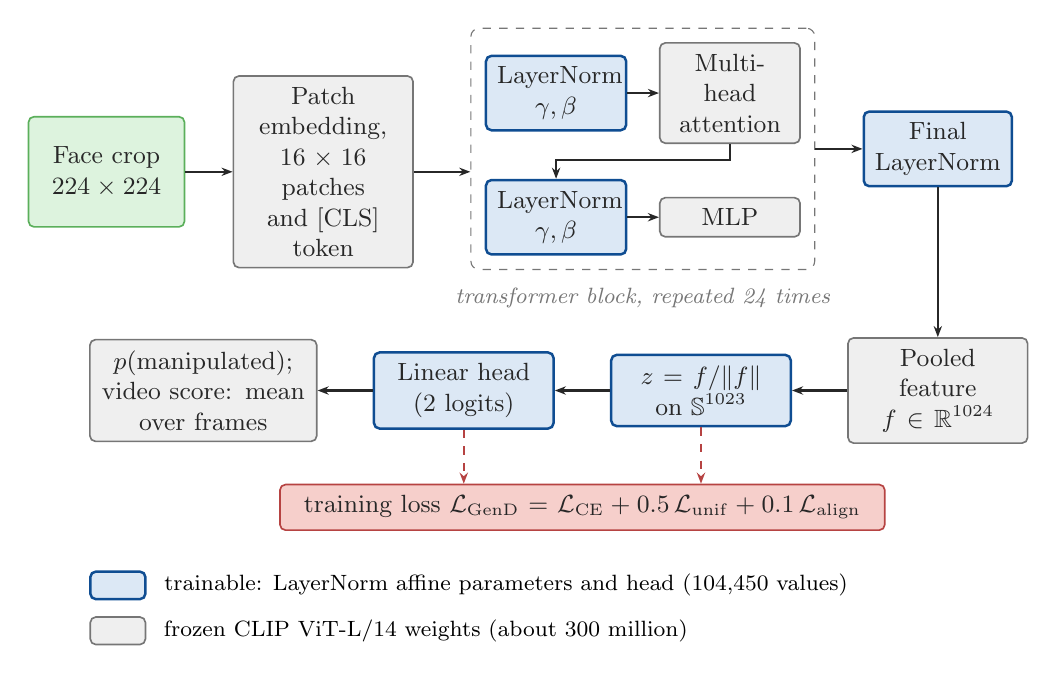
\begin{tikzpicture}[font=\small, node distance=4mm and 5mm]
\node[data, text width=1.7cm, minimum height=1.4cm] (img) {Face crop\\ $224\times224$};
\node[box, text width=2.0cm, right=6mm of img, minimum height=1.4cm] (patch) {Patch\\ embedding,\\ $16\times16$ patches\\ and [CLS] token};
\node[ours, text width=1.5cm, right=9mm of patch, yshift=10mm] (ln1) {LayerNorm\\ $\gamma,\beta$};
\node[box, text width=1.5cm, right=4mm of ln1] (att) {Multi-head\\ attention};
\node[ours, text width=1.5cm, below=6mm of ln1] (ln2) {LayerNorm\\ $\gamma,\beta$};
\node[box, text width=1.5cm, right=4mm of ln2] (mlp) {MLP};
\draw[arr] (ln1) -- (att); \draw[arr] (ln2) -- (mlp);
\draw[arr] (att.south) -- ++(0,-2mm) -| (ln2.north);
\begin{scope}[on background layer]
\node[draw=nline, dashed, rounded corners=3pt, fit=(ln1)(att)(ln2)(mlp), inner sep=5pt] (blk) {};
\end{scope}
\node[lab, below=1mm of blk] {transformer block, repeated 24 times};
\draw[arr] (img) -- (patch);
\draw[arr] (patch.east) -- (blk.west |- patch.east);
\node[ours, text width=1.6cm, right=6mm of blk] (lnf) {Final\\ LayerNorm};
\draw[arr] (blk.east |- lnf.west) -- (lnf.west);
\node[box, text width=2.0cm, below=19mm of lnf] (feat) {Pooled feature\\ $f\in\mathbb{R}^{1024}$};
\draw[arr] (lnf) -- (feat);
\node[ours, text width=2.0cm, left=7mm of feat] (norm) {$z=f/\|f\|$\\ on $\mathbb{S}^{1023}$};
\node[ours, text width=2.0cm, left=7mm of norm] (head) {Linear head\\ (2 logits)};
\node[box, text width=2.6cm, left=7mm of head] (out) {$p(\text{manipulated})$;\\ video score: mean\\ over frames};
\draw[arr] (feat) -- (norm); \draw[arr] (norm) -- (head); \draw[arr] (head) -- (out);
\node[warn, text width=7.4cm, below=7mm of $(norm.south)!0.5!(head.south)$] (loss) {training loss $\mathcal{L}_{\mathrm{GenD}}=\mathcal{L}_{\mathrm{CE}}+0.5\,\mathcal{L}_{\mathrm{unif}}+0.1\,\mathcal{L}_{\mathrm{align}}$};
\draw[arr, dashed, draw=rline] (norm.south) -- (norm.south |- loss.north);
\draw[arr, dashed, draw=rline] (head.south) -- (head.south |- loss.north);
\node[ours, minimum width=7mm, minimum height=3.5mm, inner sep=0pt, anchor=north west] (k1) at ($(out.south west |- loss.south)+(0,-5mm)$) {};
\node[right=1mm of k1, font=\footnotesize, anchor=west] {trainable: LayerNorm affine parameters and head (104{,}450 values)};
\node[box, minimum width=7mm, minimum height=3.5mm, inner sep=0pt, below=2mm of k1] (k2) {};
\node[right=1mm of k2, font=\footnotesize, anchor=west] {frozen CLIP ViT-L/14 weights (about 300 million)};
\end{tikzpicture}
\end{document}
